\chapter{ANITA \nutau regeneration paper}
\label{app:ANITA_few_author}

The paper attached in this section, ``Observing EeV neutrinos through the Earth: GZK and the anomalous ANITA events,'' outlines the software framework \texttt{TauRunner}\footnote{available at \url{https://github.com/IceCubeOpenSource/TauRunner}} and calculations surrounding \nutau regeneration from high-energy \nutau fluxes. 

The analysis has applications in constraining high-energy \nutau point-source fluxes as well as for searching for cosmogenic neutrinos. It was published in \textit{The Journal of Cosmology and Astroparticle Physics} on January 3, 2020 \citep{Safa:2019ege}.

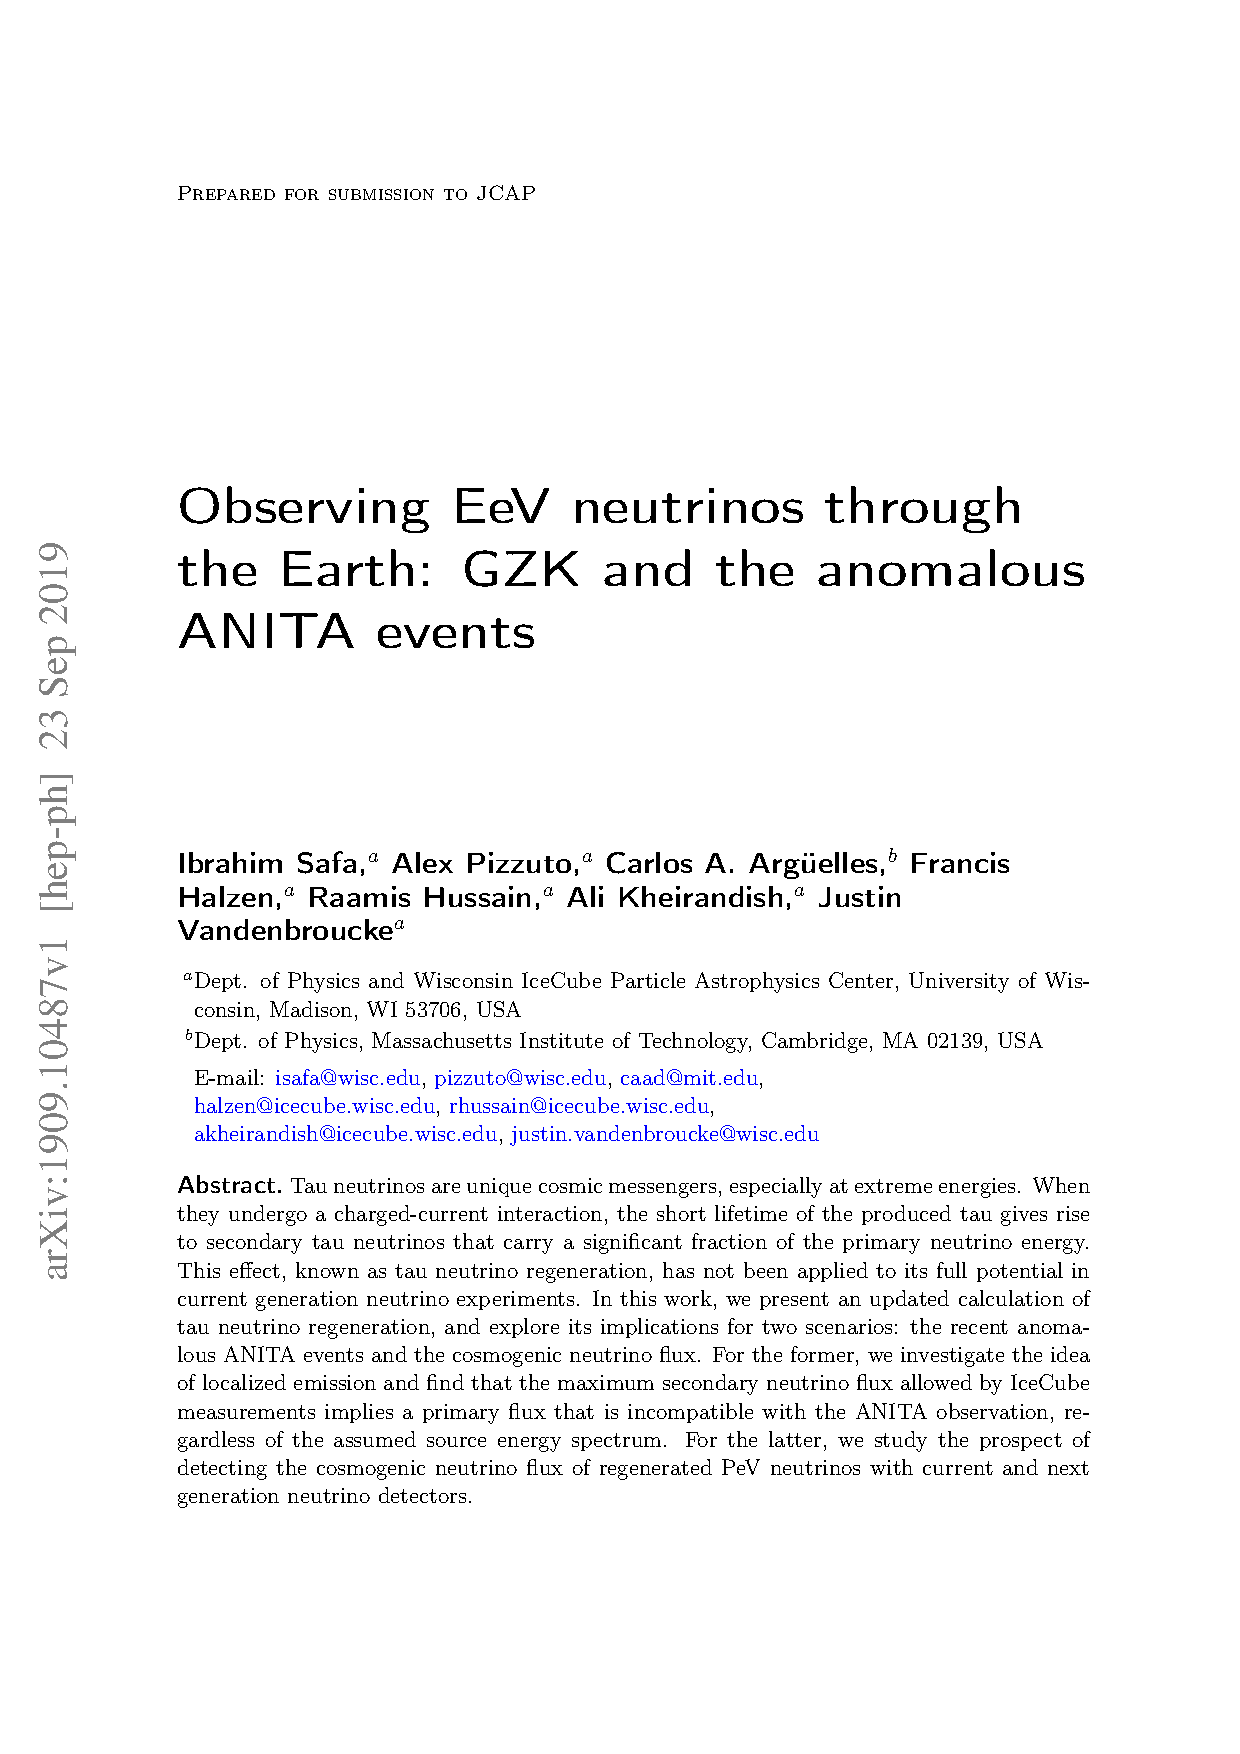
\includepdf[pages=-,pagecommand={},width=\pagewidth]{papers/ANITA_few_author_paper.pdf}